\multiplechoicestart


\spoergsmaal{Arrays}
Lad \(A[0:5] = \langle 3, 7, 1, 6, 2, 8 \rangle\) og \(B[1:4] = \langle 2, 5, 3, 1 \rangle\).
Hvad er \(A[B[3] \cdot B[1] - 4]\)?
\etsvar

\mulighederstart
\svar Værdien er \(1\) \korrekt
\svar Værdien er \(2\)
\svar Værdien er \(3\)
\svar Værdien er \(6\)
\svar Værdien er \(7\)
\svar Værdien er \(8\)
\mulighederslut
\forklaring{
Vi finder \(B[3] = 3\) og \(B[1] = 2\).
Indekset bliver \(3 \cdot 2 - 4 = 2\).
Dermed er \(A[2] = 1\).
}

\spoergsmaal{Toppunkter i array}
Hvilke indekser er toppunkter i følgende array: \(A[1:5] = [5,7,7,3,3]\)?
Husk at et index \(i\) er et toppunkt, hvis \(A[i]\) er større end eller lig alle naboelementer (hvert element har ét eller to naboelementer).
\fleresvar
\mulighederstart
\svar Indeks \(1\)
\svar Indeks \(2\) \korrekt
\svar Indeks \(3\) \korrekt
\svar Indeks \(4\)
\svar Indeks \(5\) \korrekt
\mulighederslut
\forklaring{
  Her er \(A[2] = 7\) større end \(A[1] = 5\) og lig \(A[3] = 7\),
  og \(A[3] = 7\) lig \(A[2] = 7\) og større end \(A[4] = 3\).
  Derfor er \(2\) og \(3\) toppunkter.
  Da \(A[5]=3\) kun har én nabo \(A[4]=3\), så er \(5\) også et toppunkt.
}


\spoergsmaal{Typer af grafer}
Hvilke af følgende er ord fra kursets pensum som beskriver en type af grafer eller en del af en graf?
\fleresvar
\mulighederstart
\svar knudegraf
\svar kvadratisk graf
\svar orienteret graf \korrekt
\svar træ \korrekt
\svar rute
\svar cykel \korrekt
\mulighederslut
\forklaring{
I kurset har vi stødt på orienterede grafer, træer og cykler, men de andre ord findes ikke som standard terminologi for graftyper eller -dele.
}


\spoergsmaal{Datastrukturer fra pensum}
Hvilke af følgende ord er navne på datastrukturer fra kursets pensum?
\fleresvar
\mulighederstart
\svar datanet
\svar kø \korrekt
\svar samling
\svar hashtabel \korrekt
\svar total ordning
\mulighederslut
\forklaring{
I kurset har vi lært om køer og hashtabeller.
De andre ord er ikke standard datastrukturer.
}

\spoergsmaal{Sorteringsalgoritmer fra pensum}
Hvilke af følgende er sorteringsalgoritmer fra kursets pensum?
\fleresvar
\mulighederstart
\svar insertion sort \korrekt
\svar total sort
\svar counting sort \korrekt
\svar adaptive sort
\svar linear sort
\mulighederslut
\forklaring{
Counting sort og insertion sort er klassiske sorteringsalgoritmer fra pensum.
}

\spoergsmaal{Antisymmetrisk relation}
Lad $X$ være en mængde og lad $R \subseteq X \times X$ være en relation på $X$.
Hvad betyder det at $R$ er antisymmetrisk?
\etsvar
\mulighederstart
\svar $(a,b)\in R \Rightarrow a=b$
\svar $(a,b)\in R \Rightarrow (b,a)\notin R$
\svar $(a,b) \in R \land a\neq b \Rightarrow (b,a) \notin R$ \korrekt
\svar $(a,b) \in R \land (b,c) \in R \Rightarrow (c,a) \in R$
\mulighederslut
\forklaring{
En relation $R$ er antisymmetrisk hvis $(a,b)\in R\land (b,a)\in R\Rightarrow a=b$, eller ækvivalent $(a,b) \in R \land a\neq b \Rightarrow (b,a) \notin R$.
De andre udsagn beskriver asymmetri eller unavngivne egenskaber.
}
\sideskift

\spoergsmaal{Antal delmængder}
Hvor mange delmængder har en mængde med $10$ elementer?
\etsvar
\mulighederstart
\svar $\binom{10}{2}$
\itxsvar{binom(10,2)}
\svar $\binom{2}{10}$
\itxsvar{binom(2,10)}
\svar $10!$
\svar $2^{10}$ \korrekt
\svar $10$
\mulighederslut
\forklaring{
Svaret er $2^{10}$, idet hvert element kan være med i delmængden eller ej.
}


\spoergsmaal{Antal rækkefølger}
Vi har $20$ forskellige spillekort liggende i en hat.
Vi trækker et kort uden at lægge det tilbage, og trækker så et nyt, og sådan bliver vi ved til vi har trukket $4$ kort.
Hvor mange forskellige rækkefølger af $4$ kort er der mulighed for?
\etsvar
\mulighederstart
\svar $20^4$
\svar $4^{20}$
\svar $20!/4!$
\svar $20!/16!$  \korrekt
\svar $\binom{20}{4}$
\itxsvar{binom(20,4)}
\svar $\binom{20}{16}$
\itxsvar{binom(20,16)}
\mulighederslut
\forklaring{
Vi har $20$ muligheder for første kort, dernæst $19$, så $18$ og til sidst $17$, hvilket giver $20\cdot 19\cdot 18\cdot 17=20!/16!$ i alt.
}

\spoergsmaal{Matrixudregning}
Betragt følgende matricer:
\begin{align*}
    A =
\begin{bmatrix}
2 & 1\\
0 & 3\\
1 & 2
\end{bmatrix}
\quad \text{og} \quad
B =
\begin{bmatrix}
1 & 0\\
2 & 1\\
1 & 3
\end{bmatrix}.
\end{align*}

Hvad er \(A^{T}B\)? (Her er \(A^{T}\) den transponerede af \(A\).)
\etsvar
\mulighederstart

\svar \(\displaystyle \begin{bmatrix} 3 & 9\\ 3 & 9 \end{bmatrix}\)
\itxsvar{[[3,9],[3,9]]}

\svar \(\displaystyle \begin{bmatrix} 9 & 9\\ 3 & 3 \end{bmatrix}\)
\itxsvar{[[9,9],[3,3]]}

\svar \(\displaystyle \begin{bmatrix} 9 & 3\\ 9 & 3 \end{bmatrix}\)
\itxsvar{[[9,3],[9,3]]}

\svar \(\displaystyle \begin{bmatrix} 3 & 3\\ 9 & 9 \end{bmatrix}\) \korrekt
\itxsvar{[[3,3],[9,9]]}

\mulighederslut

\forklaring{
Vi har
\begin{align*}
    A^{T} =
\begin{bmatrix}
2 & 0 & 1\\
1 & 3 & 2
\end{bmatrix}.
\end{align*}

Dermed er
\begin{align*}
A^{T}B &=
\begin{bmatrix}
2 & 0 & 1\\
1 & 3 & 2
\end{bmatrix}
\begin{bmatrix}
1 & 0\\
2 & 1\\
1 & 3
\end{bmatrix} \\
&=
\begin{bmatrix}
2\cdot1 + 0\cdot2 + 1\cdot1 & 2\cdot0 + 0\cdot1 + 1\cdot3\\
1\cdot1 + 3\cdot2 + 2\cdot1 & 1\cdot0 + 3\cdot1 + 2\cdot3
\end{bmatrix} \\
&=
\begin{bmatrix}
3 & 3\\
9 & 9
\end{bmatrix}.
\end{align*}
}

\spoergsmaal{Pseudokode}
Betragt følgende pseudokode
\begin{codebox}
\Procname{$\proc{Loop}(x)$}
\li $S \gets 0$
\li \For $i \gets 1$ \To $x$ \Do
\li \quad $S \gets S + 2i$
\li \quad $S \gets S - 1$
    \End
\li \Return S
\end{codebox}
Hvad returneres når koden kaldes med input $x=3$?
\etsvar
\mulighederstart
\svar Der returneres 6
\svar Der returneres 9 \korrekt
\svar Der returneres 11
\svar Der returneres 12
\svar Der returneres 15
\mulighederslut
\forklaring{
Vi starter med $S=0$.
\begin{itemize}
    \item Iteration \(i = 1\): $S = 0 + 2\cdot1 = 2$, derefter $S = 2 - 1 = 1$
    \item Iteration \(i = 2\): $S = 1 + 4 = 5$, derefter $S = 5 - 1 = 4$
    \item Iteration \(i = 3\): $S = 4 + 6 = 10$, derefter $S = 10 - 1 = 9$
\end{itemize}
Dermed returneres $S = 9$.
}

\spoergsmaal{Markovs Ulighed}
Lad \(X\geq 0\) være en stokastisk variabel hvor det oplyses at $\mathbb E[X]=7/2$, og lad $Y=4X$.
Hvilken øvre grænse kan vi med Markovs ulighed give for sandsynligheden af
\begin{align*}
  \Pr(Y \geq 20 )?
\end{align*}
\etsvar

\mulighederstart
\svar Den øvre grænse er \(3/4\)
\svar Den øvre grænse er \(2/3\)
\svar Den øvre grænse er \(4/5\)
\svar Den øvre grænse er \(7/10\) \korrekt
\mulighederslut

\forklaring{
Vi har at \(\mathbb{E}[Y] = 4 \cdot 7/2 = 14\).
Vi ønsker at estimere
\begin{align*}
  \Pr(Y \geq 20).
\end{align*}
Ved Markovs ulighed sætter vi
\begin{align*}
  a = \frac{20}{14} = \frac{10}{7},
\end{align*}
hvilket giver
\begin{align*}
  \Pr(Y \geq 20) \leq \frac{1}{a} = \frac{7}{10}.
\end{align*}
}
\sideskift

\spoergsmaal{Repræsentation af binært søgetræ i array}
Lad os repræsentere et binært søgetræ i et array \(A[0:n-1]\) sådan at en knude er gemt
som fire på hinanden følgende felter \(A[i:i+3]\), hvor \(A[i]\) er nøgleværdien,
og \(A[i+1], A[i+2], A[i+3]\) er pointere til hhv.\ forælder, venstre barn og højre barn.
Vi gemmer roden på felterne \(A[0:3]\).
NIL-pointeren noteres som en skråstreg: \(/\).
Hvilket af nedenstående arrays repræsenterer følgende binære søgetræ?

\begin{center}
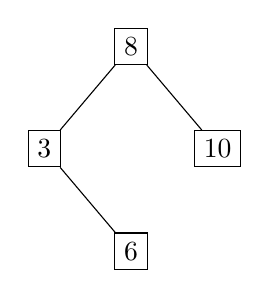
\begin{tikzpicture}[level distance=1.3cm, sibling distance=2.2cm]
  \node[draw,rectangle] {8}
    child {node[draw,rectangle] {3}
      child[missing]
      child {node[draw,rectangle] {6}}
    }
    child {node[draw,rectangle] {10}};
\end{tikzpicture}
\end{center}
\etsvar

\mulighederstart
\svar \(\langle 8, /, 4, 8, 3, 0, /, 12, 10, 0, /, /, 6, 4, /, / \rangle\) \korrekt
\svar \(\langle 8, /, 4, 8, 3, 0, 12, /, 10, 0, /, /, 6, 0, /, / \rangle\)
\svar \(\langle 8, /, 8, 4, 3, 0, 12, /, 10, 0, 12, /, 6, 4, /, / \rangle\)
\svar \(\langle 8, /, 8, 4, 3, 0, /, 12, 10, 0, 12, /, 6, 4, /, / \rangle\)
\svar \(\langle 8, /, 8, 4, 3, 0, /, 12, 10, 0, 12, /, 6, 0, /, / \rangle\)
\mulighederslut
\forklaring{
  Vi bruger blokke af fire felter per knude med indeks \(0,4,8,12\).
  \begin{itemize}
    \item Roden \(8\) ligger på \(A[0]\) med forælder \(/\), venstre barn \(4\) (knuden \(3\)) og højre barn \(8\) (knuden \(10\)).
    \item Knuden \(3\) ligger på \(A[4]\) med forælder \(0\) (roden), ingen venstre barn \((/)\) og højre barn \(12\) (knuden \(6\)).
    \item Knuden \(10\) ligger på \(A[8]\) med forælder \(0\) og ingen børn.
    \item Knuden \(6\) ligger på \(A[12]\) med forælder \(4\) og ingen børn.
  \end{itemize}
  Arrayet
  \(\langle 8, /, 4, 8, 3, 0, /, 12, 10, 0, /, /, 6, 4, /, / \rangle\)
  er det eneste, der svarer til dette træ.
}


\spoergsmaal{Pseudokode 2}
Betragt følgende pseudokode
\begin{codebox}
\Procname{$\proc{While-Loop}(x)$}
\li $y \gets 1$
\li $i \gets 0$
\li \While $i < x$ \Do
\li \quad $y \gets 2 \cdot y$
\li \quad $i \gets i + 1$
    \End
\li \Return $y$
\end{codebox}
Hvilken funktion udregner pseudokoden, når $x$ er et ikke-negativt heltal?
\etsvar
\mulighederstart
\svar $2x$
\svar $x^2$
\svar $2^x$ \korrekt
\svar $x^2+1$
\svar $x!$
\mulighederslut
\forklaring{
Variablen $y$ starter på $1$. For hver iteration ganges $y$ med $2$, og løkken kører præcis $x$ gange.
Dermed bliver slutværdien
\[
y = 1 \cdot 2^x = 2^x.
\]
Pseudokoden udregner altså funktionen $2^x$.
}

\spoergsmaal{Bredde-først søgning}
Betragt den følgende orienterede graf $G$:

\begin{center}
\begin{tikzpicture}[>=Stealth, node distance=2.4cm]
    \tikzstyle{vertex}=[circle,draw,minimum size=18pt,inner sep=0pt]
    % Nodes
    \node[vertex] (A) {$A$};
    \node[vertex,right of=A] (B) {$B$};
    \node[vertex,right of=B] (C) {$C$};
    \node[vertex,below of=A,yshift=-0.8cm] (D) {$D$};
    \node[vertex,below of=B,yshift=-0.8cm] (E) {$E$};
    \node[vertex,below of=C,yshift=-0.8cm] (F) {$F$};

    % Edges
    \draw[->] (A) to (B);
    \draw[->] (A) to (D);
    \draw[->] (B) to (C);
    \draw[->] (B) to (E);
    \draw[->] (C) to (F);
    \draw[->] (E) to (D);
\end{tikzpicture}
\end{center}

Fra hvilke startknuder vil en bredde-først søgning (BFS) finde \emph{alle} andre knuder i grafen?
Med andre ord, vælg de knuder $s\in\{A,B,\ldots,F\}$ så kaldet $\proc{BFS}(G,s)$ farver alle knuder sorte, hvor $\proc{BFS}(G,s)$ er algoritmen fra CLRS afsnit 20.2.
\fleresvar

\mulighederstart
\svar \(A\) \korrekt
\svar \(B\)
\svar \(C\)
\svar \(D\)
\svar \(E\)
\svar \(F\)
\mulighederslut
\forklaring{
  Starter vi i \(A\), kan vi nå \(B\) og \(D\). Fra \(B\) kan vi nå \(C\) og \(E\),
  og fra \(C\) kan vi nå \(F\). Dermed kan vi fra \(A\) nå samtlige knuder
  \(B, C, D, E, F\).

  Ingen af de andre knuder kan nå \(A\), og flere af dem kan kun nå et fåtal
  af de øvrige knuder. Derfor er \(A\) den eneste knude, hvorfra en BFS
  når alle andre knuder.
}


\spoergsmaal{Master Theorem}
Betragt den følgende rekursion:
\begin{align*}
    T(1) & = 1 \\
    T(n) & = 2 \cdot T(\lceil n/2 \rceil) + 3 n^{3} \quad \text{for } n \geq 2.
\end{align*}
Ved brug af Master Theorem, hvilket af følgende udsagn om \(T(n)\) er korrekt?
\etsvar

\mulighederstart
\svar \(T(n) = \Theta(n \log_{2} n)\)
\svar \(T(n) = \Theta(n^{2})\)
\svar \(T(n) = \Theta(n^{2} \log_{2} n)\)
\svar \(T(n) = \Theta(n^{3})\) \korrekt
\svar \(T(n) = \Theta(n^{3} \log_{2} n)\)
\mulighederslut
\forklaring{
Her har vi \(a = 2\), \(b = 2\) og \(f(n) = 3n^{3}\).
Dermed er
\begin{align*}
  n^{\log_{b} a} = n^{\log_{2} 2} = n.
\end{align*}
Vi ser at
\begin{align*}
  f(n) = 3n^{3} = \Omega\bigl(n^{1+\varepsilon}\bigr)
\end{align*}
for eksempel med \(\varepsilon = 2\).
Desuden gælder regularitetsbetingelsen
\begin{align*}
  a\,f(n/b)
  &= 2 \cdot 3 (n/2)^{3}
   = \frac{3}{4} n^{3}
   \le c \, n^{3}
\end{align*}
for et passende \(c < 1\) f.eks. \(\frac{3}{4}\).
Derfor er vi i case 3 af Master Theorem, og får
\begin{align*}
  T(n) = \Theta\bigl(f(n)\bigr) = \Theta(n^{3}).
\end{align*}
}


\spoergsmaal{Insertion Sort}
Betragt det følgende array \(A[1:6] = [5,2,4,6,1,3]\) og pseudokoden for \proc{Insertion-Sort} nedenfor.
Hvor mange gange bliver tallet 4 flyttet
(dvs.~skrevet et sted i $A$) under sorteringen af \(A\)?
\begin{codebox}
  \Procname{$\proc{Insertion-Sort}(A,n)$}
  \li \For $i \gets 2$ \To $n$ \Do
  \li $key \gets A[i]$
  \li $j \gets i-1$
  \li \While $j > 0$ and $A[j] > key$ \Do
  \li $A[j+1] \gets A[j]$
  \li $j \gets j-1$ \End
  \li $A[j+1] \gets key$
  \End
\end{codebox}
\etsvar
\mulighederstart
\svar Det bliver flyttet \(0\) gange
\svar Det bliver flyttet \(1\) gange
\svar Det bliver flyttet \(2\) gange 
\svar Det bliver flyttet \(3\) gange \korrekt
\svar Det bliver flyttet \(4\) gange
\mulighederslut
\forklaring{4 bliver flyttet tre gange. Først når den selv bliver indsat
(linje 7) til position 2, og så to gange mere når 1 og 3 bliver indsat foran den.}


\spoergsmaal{Max-Heap}
Du kører \proc{Build-Max-Heap} på arrayet \(A[1:7] = \langle 5, 1, 9, 3, 7, 2, 6 \rangle\).
Hvilken hob får du som resultat?
\etsvar
\mulighederstart
\svar \(\langle 9, 6, 7, 3, 2, 1, 5 \rangle\)
\svar \(\langle 9, 6, 7, 3, 1, 5, 2 \rangle\)
\svar \(\langle 9, 7, 6, 3, 1, 5, 2 \rangle\)
\svar \(\langle 9, 7, 6, 3, 1, 2, 5 \rangle\) \korrekt
\svar \(\langle 9, 7, 6, 3, 2, 1, 5 \rangle\)
\mulighederslut
\forklaring{
Start: $A = \langle 5, 1, 9, 3, 7, 2, 6 \rangle$

Efter $\proc{Max-Heapify}(A,3)$:
$\langle 5, 1, 9, 3, 7, 2, 6 \rangle$

Efter $\proc{Max-Heapify}(A,2)$:
$\langle 5, 7, 9, 3, 1, 2, 6 \rangle$

Efter $\proc{Max-Heapify}(A,1)$:
Først byttes 5 og 9:
$\langle 9, 7, 5, 3, 1, 2, 6 \rangle$

Derefter fortsætter vi fra index 3, hvor 5 byttes med 6:
$\langle 9, 7, 6, 3, 1, 2, 5 \rangle$
}
\sideskift

\spoergsmaal{Forventet Værdi}
Lad \(X_{1}, X_{2}, X_{3}\) svare til resultaterne af tre uafhængige kast med en fem-sidet terning med sider nummereret fra 1 til 5 som hver er lige sandsynlige (vi forestiller os at sådan en terning eksisterer).
Hvad er den forventede værdi af \(X_{1}\cdot X_{2}\cdot X_{3}\)?

\etsvar
\mulighederstart
\svar Den forventede værdi er 3
\svar Den forventede værdi er 5 
\svar Den forventede værdi er 15 
\svar Den forventede værdi er 25
\svar Den forventede værdi er 27 \korrekt
\mulighederslut
\forklaring{Den forventede værdi af produktet af uafhængige stokastiske variable er produktet af deres forventede værdier:
  \begin{align*}
    \mathbb{E}[X_{1}\cdot X_{2}\cdot X_{3}] =
    \mathbb{E}[X_{1}] \cdot \mathbb{E} [X_{2}] \cdot \mathbb{E} [X_{3}].
  \end{align*}
  Den forventede værdi af et enkelt kast med en fem-sidet terning er
  \begin{align*}
      \mathbb{E}[X_{i}] &=
      \frac{1+2+3+4+5}{5} = 3.
  \end{align*}
  Så 
  \begin{align*}
      \mathbb{E}[X_{1}\cdot X_{2}\cdot X_{3}] &=
      3 \cdot 3 \cdot 3 = 27.
  \end{align*}
  
}


\spoergsmaal{Hobe}
Betragt denne max-hob: $A[1:6]=\langle 99, 72, 70, 35, 7, 15\rangle$.
Vi kan indsætte nye værdier ved hjælp af \(\proc{Max-Heap-Insert}\).
Hvis vi indsætter værdien \(76\),
hvilket index ender den med at have?
\etsvar
\mulighederstart
\svar Indeks 1
\svar Indeks 2
\svar Indeks 3 \korrekt
\svar Indeks 4 
\svar Indeks 5 
\svar Indeks 6 
\svar Indeks 7 
\mulighederslut
\forklaring{Vi indsætter først 76 i index 7.
  Derefter sammenligner vi med dens forælder i position 3 (70).
  Da \(76 > 70\) bytter vi dem.
  Så sammenligner vi 76 med dens nye forælder på index 1 (99).
  Da \(76 < 99\) terminerer algoritmen, med 76 på index 3.}


\spoergsmaal{Disjunkte mængder}
Vi betragter en inddeling af tallene $\{0,1,\ldots,6\}$ i disjunkte delmængder.
Mængderne repræsenteres som en skov givet ved tabel-repræsentationen
\[
P[0:6] = \langle 2, 3, 2, 3, 2, 5, 0 \rangle,
\]
hvor \(P[i]\) angiver forælderen til element \(i\).

Hvad er mængderne?
\etsvar

\mulighederstart
\svar \(\{0,1,2\},\{3,4,5\},\{6\}\)
\svar \(\{0,1,2\},\{3\},\{4,5\},\{6\}\)
\svar \(\{0,2,4,6\},\{1,3\},\{5\}\) \korrekt
\svar \(\{0,1,2,4,6\},\{3\},\{5\}\)
\mulighederslut

\forklaring{
Vi ser at 2 er forælder til 0 og 4, og at 0 er forælder til 6, så den ene mængde er \(\{0,2,4,6\}\).
Forælderen til 1 er 3, og 5 er sin egen forælder, så de andre mængder er \(\{1,3\}\) og \(\{5\}\).
}


\spoergsmaal{Relationer}
Betragt følgende relation \(R\) på mængden af heltal \(\mathbb{Z}\):
\begin{align*}
    m R n \iff | m - n | \leq 5
\end{align*}
Hvilke egenskaber har relationen $R$?
\fleresvar

\mulighederstart
\svar antisymmetrisk
\svar symmetrisk \korrekt
\svar refleksiv \korrekt
\svar transitiv
\mulighederslut
\forklaring{Relationen er ikke antisymmetrisk, da for eksempel $0\, R\, 5$ og $5\, R\, 0$, men $0\neq 5$.
Relationen er refleksiv, da \(|m - m| = 0 \leq 5\) for alle \(m \in \mathbb{Z}\).
Relationen er symmetrisk, da \(|m - n| = |n - m|\) for alle \(m,n \in \mathbb{Z}\).
Relationen er ikke transitiv, da for eksempel $0\, R\, 5$ og $5\, R\, 10$, men \(| 0 - 10 | > 5\).}

\spoergsmaal{Kombinatorik}
10 elever skal fordeles i grupper af størrelserne 5, 3 og 2,
så hver elev er i præcis én gruppe.
Hvor mange forskellige måder kan dette gøres på?
\etsvar

\mulighederstart
\svar \(10^5\)
\svar \(10!\)
\svar \(\binom{10}{5} \cdot \binom{5}{3}\) \korrekt
\itxsvar{binom(10,5)*binom(5,3)}
\svar \(10^{5} \cdot 5^{3}\)
\svar \(5! \cdot 3! \cdot 2!\)
\svar \(\binom{10}{5} \cdot \binom{10}{3} \cdot \binom{10}{2}\)
\itxsvar{binom(10,5)*binom(10,3)*binom(10,2)}
\mulighederslut
\forklaring{
  Først vælger vi, hvilke 5 elever der skal være i gruppen på 5:
  \(\binom{10}{5}\) muligheder.
  Af de resterende 5 vælger vi 3 til tremandsgruppen:
  \(\binom{5}{3}\) muligheder.
  De sidste 2 elever udgør automatisk tomandsgruppen, så der er kun 1 mulighed tilbage.
  I alt giver det
  \(\binom{10}{5} \cdot \binom{5}{3}\) måder.
}
\sideskift

\spoergsmaal{Dijkstras algoritme}
Betragt den følgende vægtede, orienterede graf:

\begin{center}
\begin{tikzpicture}[>=Stealth, node distance=2.4cm]
  \tikzstyle{vertex}=[circle,draw,minimum size=18pt,inner sep=0pt]

  \node[vertex] (A) at (0,0) {A};
  \node[vertex] (B) at (2,1) {B};
  \node[vertex] (C) at (2,-1) {C};
  \node[vertex] (D) at (4,1) {D};
  \node[vertex] (E) at (4,-1) {E};

  \draw[->] (A) -- node[above] {1} (B);
  \draw[->] (A) -- node[below] {4} (C);
  \draw[->] (B) -- node[above] {5} (D);
  \draw[->] (B) -- node[right] {2} (C);
  \draw[->] (C) -- node[below] {1} (E);
  \draw[->] (D) -- node[right] {1} (E);
\end{tikzpicture}
\end{center}

Antag Dijkstras algoritme anvendes til at finde korteste veje fra knuden \(A\)
til alle knuder i grafen.
Angiv i hvilken rækkefølge knuderne bliver taget ud af
prioritetskøen i Dijkstras algoritme.
\etsvar

\mulighederstart
\svar \(A B C D E\)
\svar \(A B C E D\) \korrekt
\svar \(A B D C E\)
\svar  $A C B D E$
\svar \(A C B E D\)
\svar  $A C E B D$
\mulighederslut

\forklaring{
\begin{itemize}
    \item Start: \(d(A)=0\), øvrige \(\infty\)
    \item Fra \(A\): \(d(B)=1\), \(d(C)=4\) så vi vælger \(B\)
    \item Fra \(B\): \(d(C)=1+2=3\), \(d(D)=1+5=6\)
    \item Næste: \(C\) (afstand \(3\))
    \item Fra \(C\): \(d(E)=3+1=4\)
    \item Næste: \(E\) (afstand \(4\))
    \item Sidst: \(D\) (afstand \(6\))
\end{itemize}

Rækkefølgen er \(A,B,C,E,D\).
}


\spoergsmaal{Stærke sammenhængskomponenter}
Betragt den følgende orienterede graf:

\begin{center}
\begin{tikzpicture}[>=Stealth, node distance=2.2cm]
  \tikzstyle{vertex}=[circle,draw,minimum size=18pt,inner sep=0pt]

  \node[vertex] (A) at (0,0) {A};
  \node[vertex] (B) at (2,1) {B};
  \node[vertex] (C) at (2,-1) {C};
  \node[vertex] (D) at (4,1) {D};
  \node[vertex] (E) at (4,-1) {E};
  \node[vertex] (F) at (6,1) {F};
  \node[vertex] (G) at (6,-1) {G};
  \node[vertex] (H) at (8,0) {H};

  % SCC 1: A, B, C
  \draw[->] (A) -- (B);
  \draw[->] (B) -- (C);
  \draw[->] (C) -- (A);

  % SCC 2: D, E, G, H (cycle)
  \draw[->] (D) -- (E);
  \draw[->] (E) -- (H);
  \draw[->] (H) -- (D);
  \draw[->] (H) -- (D);
  \draw[->] (E) -- (G);

  % extra edges inside SCC 2 (to make it less obvious)
  \draw[->, bend left=15] (E) to (D);
  \draw[->, bend left=15] (G) to (E);

  % connections between SCCs
  \draw[->] (C) -- (D);
  \draw[->] (H) -- (F);
  \draw[->] (D) -- (F);
\end{tikzpicture}
\end{center}

Hvilken af følgende opdelinger svarer til grafens stærke sammenhængskomponenter?
\etsvar

\mulighederstart
\svar \(\{A,B,C,D,E,F,G,H\}\)
\svar \(\{A,B,C\}, \{D,E,G,H\}, \{F\}\) \korrekt
\svar \(\{A,B,C\}, \{D,E,F,G,H\}\)
\svar \(\{A,B\}, \{C,D\}, \{E,G\}, \{F,H\}\)
\svar \(\{A,B\}, \{C,D,F,H\}, \{E,G\}\)
\mulighederslut

\forklaring{
En stærk sammenhængskomponent er en maksimal mængde af knuder, hvor der findes stier begge veje mellem alle par.

\begin{itemize}
    \item \(A \to B \to C \to A\): komponent \(\{A,B,C\}\)
    \item \(D \to E \to H \to D\) og $E\to G\to E$: komponent \(\{D,E,G,H\}\)
    \item \(F\) har ingen kanter til andre knuder: komponent \(\{F\}\)
\end{itemize}

Dermed er komponenterne:
\[
\{A,B,C\}, \{D,E,G,H\}, \{F\}.
\]
}

\spoergsmaal{Kruskals algoritme}
Betragt den følgende vægtede, uorienterede graf med knuder $\{1,2,\ldots,6\}$ og kanter $\{a,b,\ldots,j\}$.
Hver kant er mærket på formen \(\alpha:x\), hvor \(\alpha\) er kantens navn og \(x\) er dens vægt.

Vi anvender Kruskals algoritme til at finde et mindste udspændende træ i grafen.
Kanter med samme vægt behandles i alfabetisk orden efter deres kantnavn.
Hvilke kanter indgår i det mindste udspændende træ, som algoritmen finder?
\etsvar

\begin{center}
\begin{tikzpicture}[>=Stealth, node distance=2.4cm]
  \tikzstyle{vertex}=[circle,draw,minimum size=18pt,inner sep=0pt]

  \node[vertex] (A) at (0,1.5) {$1$};
  \node[vertex] (B) at (2,3) {$2$};
  \node[vertex] (C) at (2,0) {$3$};
  \node[vertex] (D) at (8,3) {$4$};
  \node[vertex] (E) at (8,0) {$5$};
  \node[vertex] (F) at (5,1.5) {$6$};

  \draw[-] (A) -- node[above left] {\(a:1\)} (B);
  \draw[-] (A) -- node[below left] {\(b:2\)} (C);
  \draw[-] (B) -- node[left] {\(c:2\)} (C);

  \draw[-] (B) -- node[above] {\(d:3\)} (D);
  \draw[-] (C) -- node[below] {\(e:3\)} (E);
  \draw[-] (D) -- node[below right] {\(f:2\)} (F);
  \draw[-] (E) -- node[above right] {\(g:2\)} (F);
  \draw[-] (D) -- node[right] {\(h:1\)} (E);

  \draw[-] (C) -- node[above left] {\(i:4\)} (F);
  \draw[-] (B) -- node[below left] {\(j:5\)} (F);
\end{tikzpicture}
\end{center}

\mulighederstart
\svar \(\{a,b,d,f,h\}\) \korrekt
\svar \(\{a,b,e,f,h\}\)
\svar \(\{a,c,d,f,h\}\)
\svar \(\{a,c,e,f,h\}\)
\svar \(\{a,c,d,g,h\}\)
\mulighederslut

\forklaring{
Kanterne behandles i stigende orden efter vægt, og ved samme vægt i alfabetisk orden:
\[
a:1,\ h:1,\ b:2,\ c:2,\ f:2,\ g:2,\ d:3,\ e:3,\ i:4,\ j:5.
\]

Vi gennemgår dem i denne rækkefølge:
\begin{itemize}
    \item \(a\) vælges: forbinder \(1\) og \(2\)
    \item \(h\) vælges: forbinder \(4\) og \(5\)
    \item \(b\) vælges: forbinder \(1\) og \(3\)
    \item \(c\) fravælges: ville danne en cykel mellem \(1,2,3\)
    \item \(f\) vælges: forbinder \(4\) og \(6\)
    \item \(g\) fravælges: ville danne en cykel mellem \(4,5,6\)
    \item \(d\) vælges: forbinder komponenterne \(\{1,2,3\}\) og \(\{4,5,6\}\)
\end{itemize}

Nu har vi valgt 5 kanter, hvilket er nok til et udspændende træ på 6 knuder.
Det mindste udspændende træ består derfor af kanterne
\[
\{a,b,d,f,h\}.
\]
}


\multiplechoiceslut

\label{page:last}
